In addition using the 21\,cm line to characterize the EoR, intensity mapping of the
\lya\ transition of neutral hydrogen would provide a wealth of information about
the state of reionization. The \lya\ line has been shown to be a tracer of high-redshift
galaxies and the bubble of ionized gas around them in \cite{2013ApJ...763..132S} and \cite{2014ApJ...786..111P}.
A number of experiments look to probe reionization through the \lya\ line, but the
largest experiment of its kind planned so far is that of the Spectro-Photometer
for the History of the Universe, Epoch of Reionization, and Ices Explorer (SPHEREx),
\cite{2014arXiv1412.4872D}.

\begin{figure}[th]
	\centering
	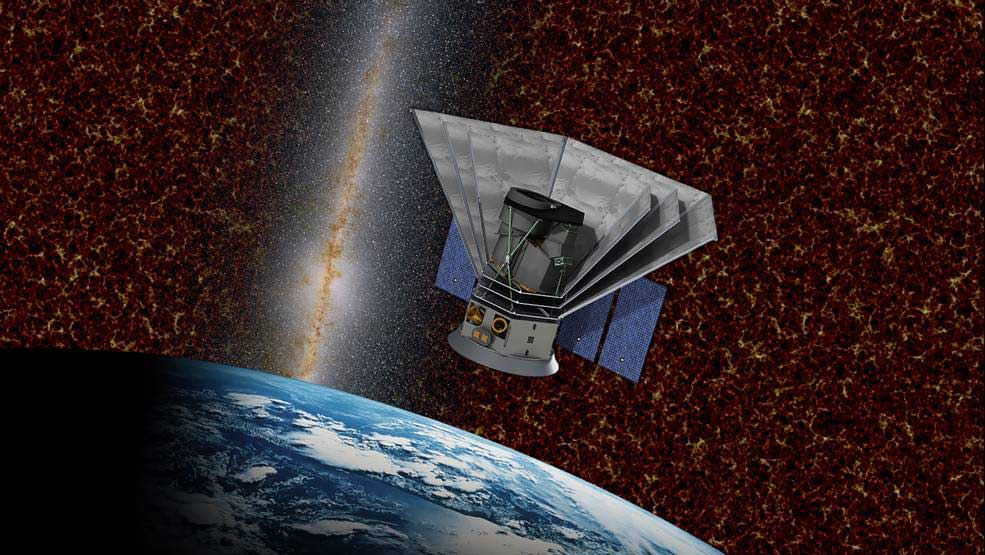
\includegraphics[width=0.95\textwidth]{spherex.jpg}
	\caption[SPHEREx Instrument]{Simulated image of the SPHEREx probe in orbit.}
	\label{fig:spherex}
\end{figure}

SPHEREx is a near-infrared, space-based observatory whose primary science goal is to perform
an all-sky survey in near-infrared bands of 450 million galaxies to constrain the
physics of inflation using the large-scale structure of these galaxies. While not
the primary goal of the mission, SPHEREx also looks to do intensity mapping of the
\lya\ line to study the origin and evolution of early galaxies. With a target launch
date set for December 2023, SPHEREx may provide the very first \lya\ intensity mapping
measurements during reionization. Given its superior sensitivity, SPHEREx should
be able to detect these EoR fluctuations over the redshift range $z \approx 6 - 8$.
